\chapter{Machine Learning}%
\label{ch:ml}

The next chapter is somewhat of a diversion from the physics discussed so far.
It will focus on techniques in machine learning which are often referred to in
High Energy Physics as a Multi-variate Analysis (MVA). The reason for this
diversion is that these techniques have become very widespread in the field,
they are used in several of the reconstruction and selection algorithms that are
used to obtain the events on which the analysis is performed. Furthermore an MVA
is used to obtain the distribution that acts as the final discriminant for the
analysis, and machine learning techniques are also used to model the
backgrounds. Given how widespread the use of these techniques is in the analysis
it makes sense to describe them before diving into the details.

The two main algorithms used are Boosted Decision Trees (BDTs) and Neural
Networks (NNs) which will be described in sections~\ref{sec:bdts}
and~\ref{sec:neural-networks} respectively. These algorithms are used in many
places outside High Energy Physics and so rather than referring to individual
pieces of data that enter into the algorithm as an event, in this chapter they
will be referred to as an example. This terminology comes from the fact that in
general these algorithms must be shown a large number of examples before they
are suitable ``trained'' for their purpose, and that in general those examples
could be data that represent anything. Both of these algorithms can be operated
in classification or regression modes. The main difference between these modes
is that classification mode provides a score for each of a given number of
classes which can be interpreted as a probability that a given example belongs
to the given class, whereas regression outputs a single number per example whose
interpretation depends on the problem.

Both algorithms can be written as a function of some inputs $\vec{x}$, some
weights to be found during training $\vec{w}$, and a set of hyper-parameters
$\vec{\theta}$ as follows
\begin{equation}
  F(\vec{x}, \vec{w}, \vec{\theta} \,) = \vec{y},
  \label{eq:ml-general}
\end{equation}
where $\vec{y}$ is a vector whose outputs correspond to each class in a
classification problem. If the algorithm is set up for a regression problem then
the output will just be one number. The hyper-parameters control the behaviour
of the algorithm in question and are set by hand in advance of training.
Training either algorithm involves an iterative process where at each iteration
the function is evaluated for the current set of weights, the outputs are
compared against some truth labels $\vec{t}$ via the computation of a loss
function. Based on the value of the loss function the weights are then updated
according to the given algorithm. It is therefore vital that firstly these truth
labels are available for the data on which one wants to train (e.g. train on
simulated predictions rather than real data) and secondly that the examples are
split into a training and testing set so that the set which is used to
iteratively update weights is not the same set that performance is evaluated on.
This avoids over-fitting to any noise in a given set, though this problem is not
circumvented entirely and over-fitting will be addressed for specific algorithms
in the sections ahead.

\section{Boosted Decision Trees}%
\label{sec:bdts}
We will start by discussing a decision tree for a classification problem.
Decision trees have a structure as in figure~\ref{fig:bdt}, which shows a tree
dividing examples into two classes, red and blue.
\begin{figure}[h]
  \centering
  \begin{tikzpicture}
    \draw [very thick] plot [smooth] coordinates {(-5,-3) (5,3)};
    \draw [very thick] plot [smooth] coordinates {(-5, 3) (5,-3)};
  \end{tikzpicture}
  \caption{The structure of a decision tree.}
  \label{fig:bdt}
\end{figure}


Each circular node in the tree represents a cut on one of a number of variables
provided as input to the algorithm. The tree is read top to bottom with each
node being followed by two edges branching left and right that represent the
path taken by examples which pass or fail the cut respectively. Square nodes
represent that the termination criteria have been reached and that events in
these nodes have been classified according to the colour of the node. The
variable chosen at each node is optimised in order to maximise a criteria
related to the separation of classes.  For a problem containing two classes a
common separation criteria is the Gini index,
\begin{equation}
  G = p(1-p),
  \label{eq:gini}
\end{equation}
where p is the purity of a chosen class that one wants to maximise.

A decision tree by itself is able to separate examples into a number of classes,
however a single tree is prone to over--training. Over--training is the term
used to describe the phenomena where a classifier learns from statistical
fluctuations in the data rather learning a generalised separation boundary
between classes. The reason that decision trees are susceptible to this is that
if two variables yield a similar separation criteria then a fluctuation in the
training data may lead to the choice of one variable over another for a
particular node, this choice will lead to a very different tree structure than
if the fluctuation were not present.

In order to mitigate the over--training tendencies of decision trees they are
often used in an ensemble algorithm such as bagging~\cite{bagging}
or boosting~\cite{boosting}. Here only boosting will be discussed. Ensembles of
decision trees are often referred to as random forests. Boosting works by
training a sequence of trees, weighting misclassified events from a tree so that
they have more influence over the structure of the next tree in the sequence.
The final classification of any given example is a weighted average over all
trees, this can be weighted by the overall accuracy of each tree, but in general
can take any weighted average.

\subsection{Gradient Boosting}

Gradient boosting is the name of an optimisation algorithm that takes the
concept of boosting and combines it with the gradient descent algorithm. A
pictographic representation of gradient descent for a regression problem can be
seen in figure~\ref{fig:grad-desc.}
\begin{figure}[ht]
  \centering
  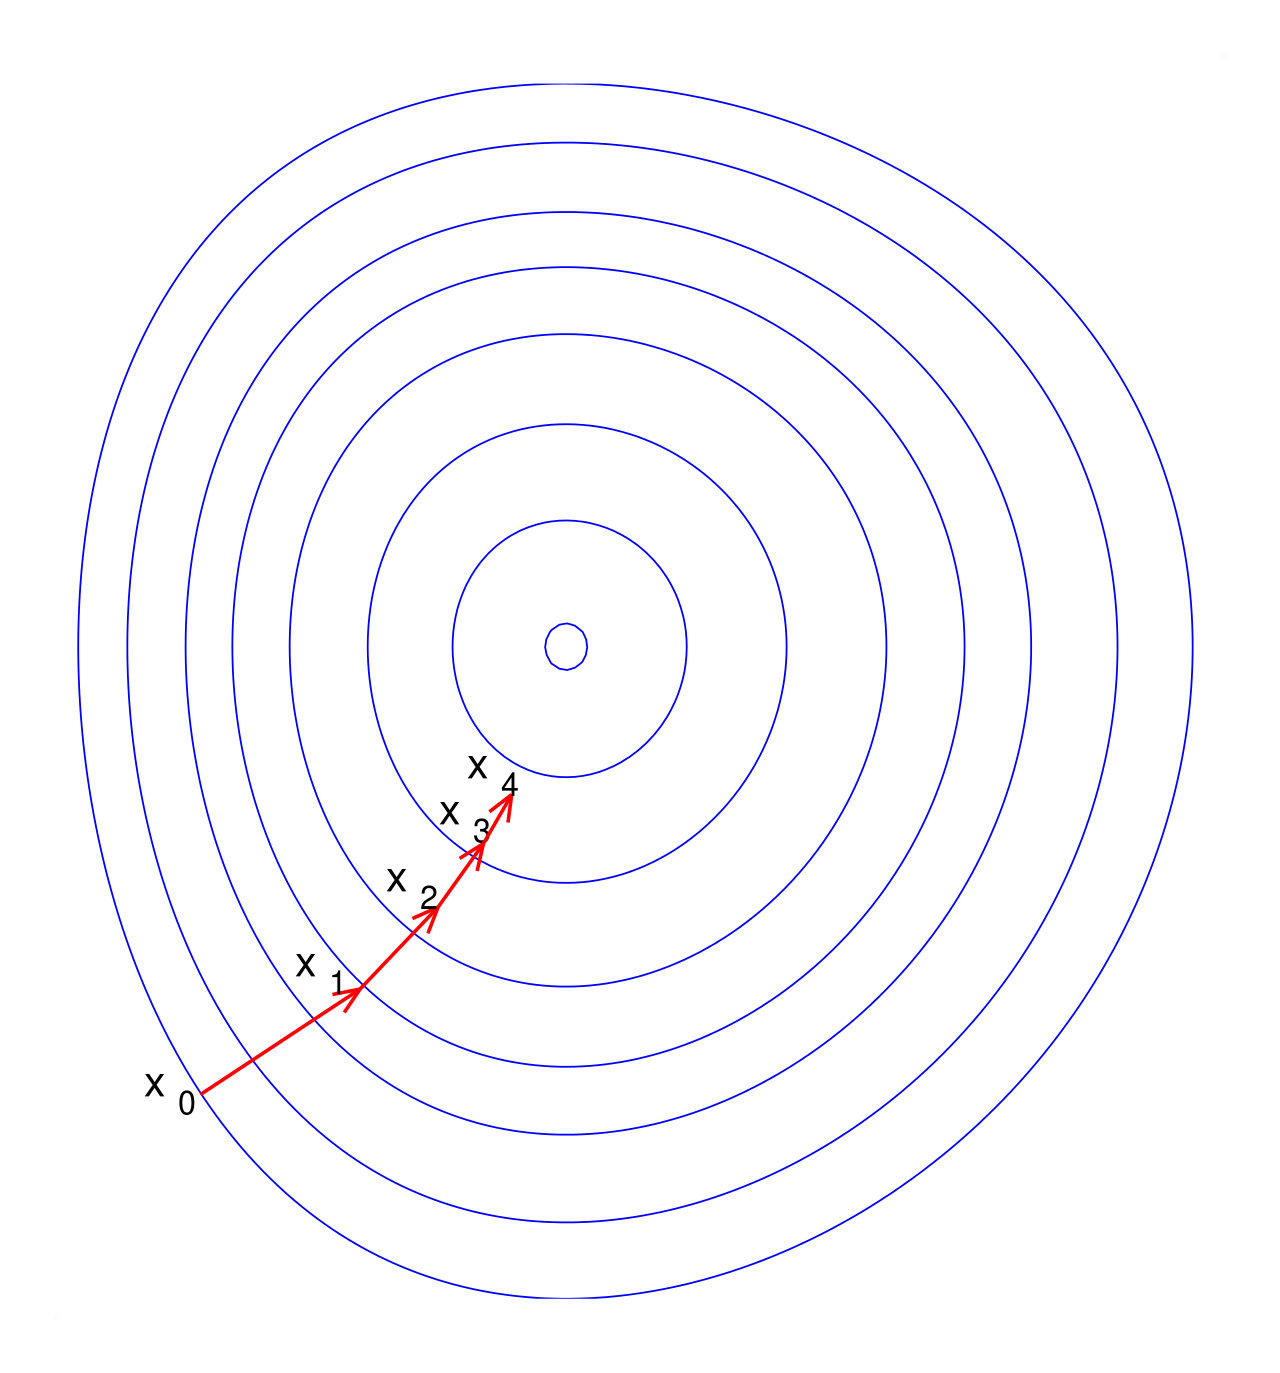
\includegraphics[width=.6\textwidth]{gradient-descent}
  \caption[An illustration of gradient descent.]{An illustration of the gradient
    descent algorithm. The blue lines represent level sets of a function, sets
    of points that have the same gradient. The $x$'s represent where in along
    the function the algorithm is at a given step with the steps numbered 0 to
    4.}
  \label{fig:grad-desc}
\end{figure}
  
The basic principle of gradient descent is to find the minimum of some
multi-variable function by taking the derivative of the function around some
starting point in the space and moving in the direction of the negative
gradient. This process is repeated iteratively until some termination criteria
is reached. In machine learning gradient descent is most often applied to the
loss function which describes the discrepancy between the predictions of a model
$\vec{y}$ and the truth labels $\vec{t}$. For a loss written as
\begin{equation}
  \mathcal{L}(\vec{y}, \vec{t} \,),
\end{equation}
the predictions and the labels define a point in the space around which the
function must be locally differentiable, it is hard to determine where these
points will be before training an algorithm on a given dataset and so in general
a loss is chosen that is differentiable everywhere.

Considering now a boosted decision tree that has a number of iterations for each
of which a decision tree is constructed using the Gini index. The model can be
written as
\begin{equation}
  F_i(\vec{x}),
\end{equation}
at a given iteration and is evolved by the addition of a single decision tree as
\begin{equation}
  F_i({\vec{x}}) + d(\vec{x}) = F_{i+1}(\vec{x}),
\end{equation}
the decision tree which is added is found by taking the negative gradient of the
loss computed at the previous iteration
\begin{equation}
  d{\vec{x}} = - \frac{\partial \mathcal{L}(F_i, \vec{t} \,)}{\partial F}.
\end{equation}
This is process is known as gradient boosting. Each decision tree is known as a
weak learner, by evolving the overall model by stepping in the direction of the
negative gradient of the loss calculated on the predictions of the model at the
current stage the algorithm aims to correct for past mistakes.

BDT Hyper-parameters.

\section{Neural Networks}%

\label{sec:neural-networks}

Like boosted decision trees neural networks can be described as a function of
input data, weights and hyper-parameters $F(\vec{x}, \vec{w}, \vec{\theta} \,)$.
Unlike BDTs neural networks can vary a lot more in their structure, the
hyper-parameters of these algorithms allow for much finer control over the
behaviour of the function as an estimator. The basic structure of a neural
network is shown in figure~\ref{fig:nn}.  The building blocks of the NN resemble
Fisher discriminants~\cite{Fisher} and take the form
\begin{equation}
a_j = \sum_{i=1}^{d} w_{ji}x_{i} + w_{j0},
\label{eq:fisher}
\end{equation}
where the $w_{ji}$ terms are known as weights and the $w_{j0}$ as biases, these
constructions are called activations. It would be remiss of me to cite the works
of Fisher without condemning his participation in the field of eugenics, but I
leave the citation here as a reminder that as scientists we have a
responsibility to society to pursue causes for good. Neural network models are
inspired by neurons in the brain, who fire when some threshold of
neuro--transmitting chemical is reached~\cite{biology} and are linked up in
intricate ways to manifest complex behaviours. In order to take activations and
give them a behaviour similar to neurons they must be passed through an
activation function, denoted $\mathcal{H}$, which gives the threshold effect
\begin{equation}
h_j = \mathcal{H}(a_j).
\label{eq:hiddenunit}
\end{equation}
These are similar to Rosenblatt's original perceptron~\cite{Rosenblatt} with the
difference that $\mathcal{H}$ must be differentiable whereas the perceptron used
a step function.

All neural networks are made of layers, and have an input layer which is a
vector of input data and an output layer, a vector whose size relates to the
predictions being made. Layers inbetween these two are called hidden layers and
are made of the units $h_j$ (known as hidden units). The most simple neural
network has a single hidden layer. This model can be written as
\begin{equation}
F(\vec{x},\vec{w}, \vec{\theta}) = \mathcal{O} \Bigg( \sum_{j=1}^{m} w_{kj}^{(2)}
\mathcal{H} \Bigg( \sum_{i=1}^{d} w_{ji}^{(1)} x_{i} + w_{j0}^{(1)} \Bigg) + w_{k0}^{(2)} \Bigg).
\label{eq:basicnn}
\end{equation}
where the superscript number in brackets labels the layer to which parameters
belong. The hyper-parameters $\vec{theta}$ here are the choice of activation
function $\mathcal{H}$, output function $\mathcal{O}$, number of hidden units
$m$ and the number of hidden layers (just one here).

The output function $\mathcal{O}$ must have properties that allow us to
interpret the outputs of the network as probabilistic. A common choice of output
function for classification problems is the softmax function
\begin{equation}
  \mathcal{O}(z)_k = p(k|\vec{x}) = \frac{exp(z_k)}{\sum_{i=1}^kexp(z_i)}
  \label{eq:softmax}
\end{equation}
where $z$ merely denotes the argument of the output function. This function
gives the probability of being an example belonging to class $k$ given the data
$\vec{x}$ where there are $k$ possible classes.

\par Now it is our goal to generalise this network function to one not only of
an arbitrary number of hidden layers but also such that each hidden layer can be
of arbitrary size and have an arbitrary activation function. For this purpose,
networks will now be described in terms of the number of hidden layers, instead
of the number of layers that contain adaptive parameters (hidden plus output) as
before. We may start by writing a function for a network of two hidden layers
\begin{equation}
y_k(\vec{x},\vec{w}) = \mathcal{O} \Bigg( \sum_{j_{2}=0}^{m_{2}} w_{kj_{2}} \mathcal{H}_{2} 
\Bigg( \sum_{j_{1}=0}^{m_{1}} w_{j_{2}j_{1}} \mathcal{H}_{1} \Bigg( \sum_{i=0}^{d} w_{j_{1}i} x_{i} \Bigg) \Bigg) \Bigg).
\label{eq:2layer}
\end{equation}
In order to arive at the two layer function \eqref{eq:2layer} the same process
was used as for the original network function \eqref{eq:basicnn}. Now there are
two activation functions and hidden layer sizes denoted $m$. Clearly adding a
layer to the network simply involves repeated application of this process and
picking up the required number of additional parameters. A function for a
network of $n$ hidden layers may therefore be written as
\begin{equation}
y_k(\vec{x},\vec{w}) = \mathcal{O} \Bigg( \sum_{j_{n}=0}^{m_{n}} w_{kj_{n}}
\mathcal{H}_{n} \Bigg( \dots \mathcal{H}_2  \Bigg( \sum_{j_{1}=0}^{m_{1}} w_{j_{2}j_{1}} 
\mathcal{H}_{1} \Bigg( \sum_{i=0}^{d} w_{j_{1}i} x_{i} \Bigg) \Bigg) \dots \Bigg) \Bigg)
\label{eq:fullnn}
\end{equation}
where there are $n$ different versions of the activation function and hidden
layer size. Our new hidden units obey the following notation
\begin{equation}
h_{nj} = \mathcal{H}_n(a_j)
\label{eq:newhiddenunits}
\end{equation}
eliminating the need for the superscript labelling of layer. The new labelling
identifies hidden layer by the left-hand index of the hidden unit or the
right-hand hidden layer of the weights and biases. In equation \eqref{eq:fullnn}
the hidden units are shown in their expanded form and distinguished by the fact
that their $j$ indices take on the subscript of $n$ corresponding to the layer
they belong to. Figure \ref{fig:fullnn} depicts a network of $n$ hidden layers,
as described in equation \eqref{eq:fullnn} except that every hidden layer is
depicted with the same size $m$.

\tikzset{%
  every neuron/.style={
    circle,
    minimum size=22pt,
    draw
  },
  neuron missing/.style={
    draw=none, 
    scale=3,
    text height=0.3cm,
    execute at end node=\color{black}\tiny{$\vdots$}
  },
}

\begin{figure}[hbtp]
  \centering
  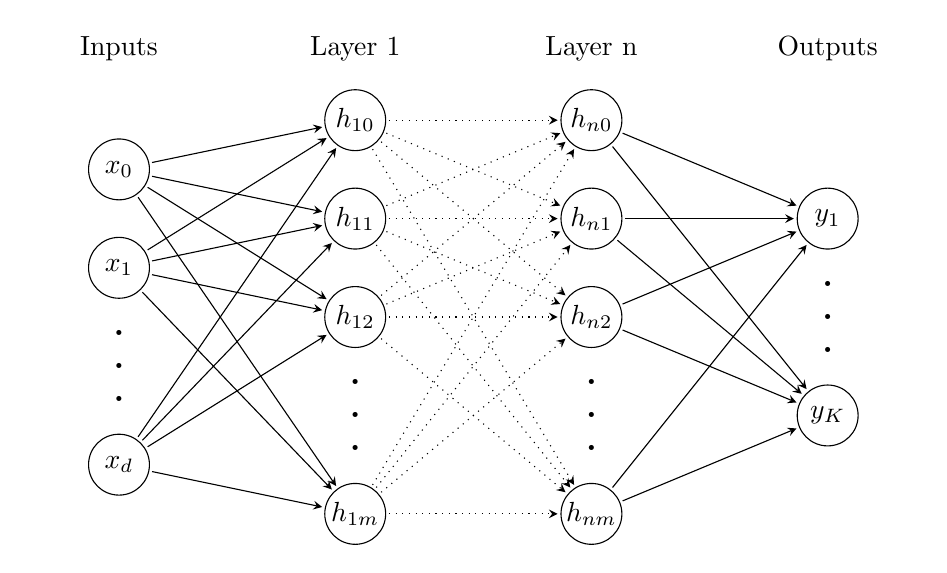
\begin{tikzpicture}[x=1.5cm, y=1.25cm, >=stealth]
    
    \foreach \m/\l [count=\y] in {1,2,missing,3}
    \node [every neuron/.try, neuron \m/.try] (input-\m) at (0,2-\y) {};

    \foreach \m [count=\y] in {1,2,3,missing,4}
    \node [every neuron/.try, neuron \m/.try ] (hidden1-\m) at (2,2.5-\y) {};

    \foreach \m [count=\y] in {1,2,3,missing,4}
    \node [every neuron/.try, neuron \m/.try ] (hidden2-\m) at (4,2.5-\y) {};

    \foreach \m [count=\y] in {1,missing,2}
    \node [every neuron/.try, neuron \m/.try ] (output-\m) at (6,1.5-\y) {};

    \foreach \l [count=\i] in {0,1,d}
    \node at (input-\i.center) {$x_{\l}$};

    \foreach \l [count=\i] in {0,1,2,m}
    \node at (hidden1-\i.center) {$h_{1\l}$};

    \foreach \l [count=\i] in {0,1,2,m}
    \node at (hidden2-\i.center) {$h_{n\l}$};

    \foreach \l [count=\i] in {1,K}
    \node at (output-\i.center) {$y_\l$};

    \foreach \i in {1,...,3}
    \foreach \j in {1,...,4}
    \draw [->, shorten <=1pt, shorten >=1pt] (input-\i) -- (hidden1-\j);

    \foreach \i in {1,...,4}
    \foreach \j in {1,...,4}
    \draw [dotted, ->, shorten <=1pt, shorten >=1pt] (hidden1-\i) -- (hidden2-\j);

    \foreach \i in {1,...,4}
    \foreach \j in {1,...,2}
    \draw [->, shorten <=1pt, shorten >=1pt] (hidden2-\i) -- (output-\j);

    \foreach \l [count=\x from 0] in {Inputs, Layer 1, Layer n, Outputs}
    \node [align=center, above] at (\x*2,2) {\l};
  \end{tikzpicture}
  \caption[A depiction of a neural network.]{A more complex neural network
    containing an input layer of $d$ nodes corresponding to data of dimensionality
    $d$, $n$ hidden layers of $m$ hidden units each $h_{ij}$ (where $i$ indexes
    hidden layer and $j$ indexes a particular unit) and an output layer of $K$
    predictive units $y_k$.}
  \label{fig:nn}
\end{figure}
There are now a great deal of parameters that we have to keep track of. It
is therefore important to distinguish between adaptive parameters and the
parameters which we must pick by hand, known as hyper-parameters. A relationship
can be written between the number of hidden layers $n$, and the number of
hyper-parameters, as follows
\begin{equation}
\text{\# of hyper-parameters} = 2n + 1.
\label{eq:hyper}
\end{equation}
As previously stated there are simply $n$ lots of activation functions and $n$
hidden layers to determine a size for. Often it is sufficient to set all
activation functions to the same function, and in this work all hidden layers
share the same size for simplicity. The adaptive parameters are far more
numerous, and will be optimised by means of a training algorithm. In TensorFlow
the variable object is choice for implementing the adaptive parameters as
training algorithms in the software will update them by default. The adaptive
parameters are initialised randomly from a Gaussian distribution resulting in
poor predictive power to begin with. In order to improve this some figure of
merit, known as a loss function, must be used in order for the training
algorithm to measure quantitatively the performance of the NN. We also must
provide the algorithm with a dataset to train on, complete with a set of targets
or labels that, for the training set, reveal the correct classification for each
entry. Due to the this requirement, methods such as these are referred to as
supervised learning methods. A natural loss function one may use to describe the
error of the model given a current set of adaptive parameters is sum-of-squares
error
\begin{equation}
E(\vec{w}) = \frac{1}{2}\sum_{n=1}^{N}(y(\vec{x}_n, \vec{w}) - t_n)^2
\label{eq:sumofsquares}
\end{equation}
where $t_n$ are the targets for the given data entries $\vec{x}_n$.
Minimising this function with some algorithm does work in practice, however it
has been shown that, using
\begin{equation}
E(\vec{w}) = - \sum_{n=1}^{N} \Bigg (t_n \ln (y_n) + (1-t_n) \ln (1-y_n) \Bigg)
\label{eq:xentropy}
\end{equation}
known as cross-entropy, is faster and more generalised \cite{XEntropySimard}
(further discussion on generalisation in section \ref{sec:generalisation}). The
particular training algorithm that will be used to update parameters in this
report is known as adaptive moment estimation or ADAM \cite{ADAMOpt}. ADAM is a
variant of the gradient descent algorithm, which is widely used and has spawned
many other variants \cite{GDOverview}. The reasons for picking between ADAM and
vanilla gradient descent are given in chapter \ref{ch:netarch}.

\tikzset{%
  every neuron/.style={
    circle,
    minimum size=22pt,
    draw
  },
  neuron missing/.style={
    draw=none, 
    scale=3,
    text height=0.3cm,
    execute at end node=\color{black}\tiny{$\vdots$}
  },
}

\begin{figure}[hbtp]
  \centering
  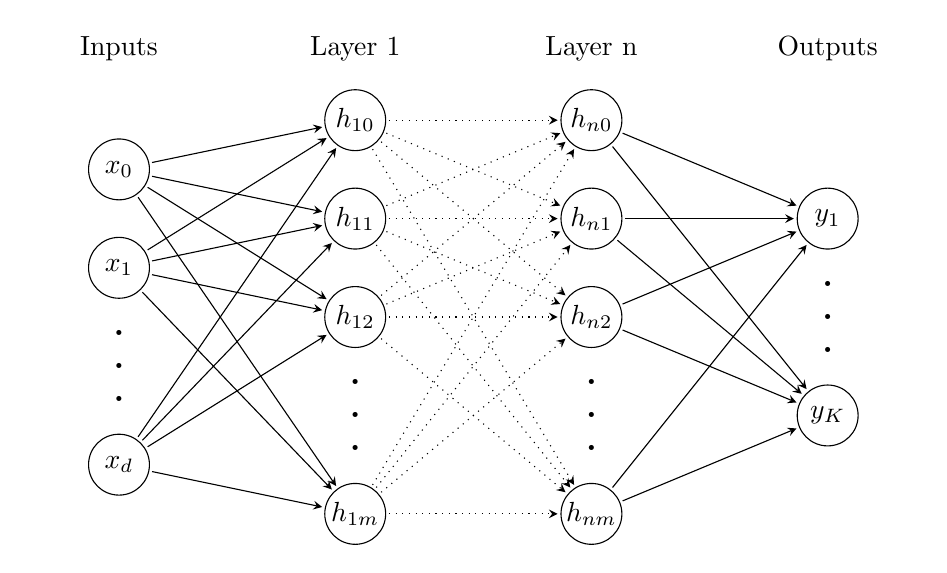
\begin{tikzpicture}[x=1.5cm, y=1.25cm, >=stealth]
    
    \foreach \m/\l [count=\y] in {1,2,missing,3}
    \node [every neuron/.try, neuron \m/.try] (input-\m) at (0,2-\y) {};

    \foreach \m [count=\y] in {1,2,3,missing,4}
    \node [every neuron/.try, neuron \m/.try ] (hidden1-\m) at (2,2.5-\y) {};

    \foreach \m [count=\y] in {1,2,3,missing,4}
    \node [every neuron/.try, neuron \m/.try ] (hidden2-\m) at (4,2.5-\y) {};

    \foreach \m [count=\y] in {1,missing,2}
    \node [every neuron/.try, neuron \m/.try ] (output-\m) at (6,1.5-\y) {};

    \foreach \l [count=\i] in {0,1,d}
    \node at (input-\i.center) {$x_{\l}$};

    \foreach \l [count=\i] in {0,1,2,m}
    \node at (hidden1-\i.center) {$h_{1\l}$};

    \foreach \l [count=\i] in {0,1,2,m}
    \node at (hidden2-\i.center) {$h_{n\l}$};

    \foreach \l [count=\i] in {1,K}
    \node at (output-\i.center) {$y_\l$};

    \foreach \i in {1,...,3}
    \foreach \j in {1,...,4}
    \draw [->, shorten <=1pt, shorten >=1pt] (input-\i) -- (hidden1-\j);

    \foreach \i in {1,...,4}
    \foreach \j in {1,...,4}
    \draw [dotted, ->, shorten <=1pt, shorten >=1pt] (hidden1-\i) -- (hidden2-\j);

    \foreach \i in {1,...,4}
    \foreach \j in {1,...,2}
    \draw [->, shorten <=1pt, shorten >=1pt] (hidden2-\i) -- (output-\j);

    \foreach \l [count=\x from 0] in {Inputs, Layer 1, Layer n, Outputs}
    \node [align=center, above] at (\x*2,2) {\l};
  \end{tikzpicture}
  \caption[A depiction of a neural network.]{A more complex neural network
    containing an input layer of $d$ nodes corresponding to data of dimensionality
    $d$, $n$ hidden layers of $m$ hidden units each $h_{ij}$ (where $i$ indexes
    hidden layer and $j$ indexes a particular unit) and an output layer of $K$
    predictive units $y_k$.}
  \label{fig:nn}
\end{figure}
\section{Parametrised Neural Networks}%
\label{sec:param-neural-nets}
Parametrised neural networks take extra inputs equal to the number of relevant
parameters, as seen in figure~\ref{fig:pnn}.
% UNUSED
% \begin{figure}[hbtp]
% \begin{center}
% \begin{tikzpicture}[x=1.5cm, y=1.25cm, >=stealth]

% \foreach \m/\l [count=\y] in {1,2,missing,3}
%   \node [every neuron/.try, neuron \m/.try] (input-\m) at (0,2-\y) {};

% \foreach \m [count=\y] in {1,2,3,missing,4}
%   \node [every neuron/.try, neuron \m/.try ] (hidden1-\m) at (2,2.5-\y) {};

% \foreach \m [count=\y] in {1,2,3,missing,4}
%   \node [every neuron/.try, neuron \m/.try ] (hidden2-\m) at (4,2.5-\y) {};

% \foreach \m [count=\y] in {1,missing,2}
%   \node [every neuron/.try, neuron \m/.try ] (output-\m) at (6,1.5-\y) {};

% \foreach \l [count=\i] in {0,1,d}
%   \node at (input-\i.center) {$x_{\l}$};

% \foreach \l [count=\i] in {0,1,2,m}
%   \node at (hidden1-\i.center) {$h_{1\l}$};

%   \foreach \l [count=\i] in {0,1,2,m}
%   \node at (hidden2-\i.center) {$h_{n\l}$};

% \foreach \l [count=\i] in {1,K}
%   \node at (output-\i.center) {$y_\l$};

% \foreach \i in {1,...,3}
%   \foreach \j in {1,...,4}
%     \draw [->, shorten <=1pt, shorten >=1pt] (input-\i) -- (hidden1-\j);

% \foreach \i in {1,...,4}
%   \foreach \j in {1,...,4}
%     \draw [dotted, ->, shorten <=1pt, shorten >=1pt] (hidden1-\i) -- (hidden2-\j);

% \foreach \i in {1,...,4}
%   \foreach \j in {1,...,2}
%     \draw [->, shorten <=1pt, shorten >=1pt] (hidden2-\i) -- (output-\j);

% \foreach \l [count=\x from 0] in {Inputs, Layer 1, Layer n, Outputs}
%   \node [align=center, above] at (\x*2,2) {\l};

% \end{tikzpicture}
% \caption{A more complex neural network containing an input layer of $d$ nodes corresponding to data of dimensionality $d$, $n$ hidden layers of $m$ hidden units each $h_{ij}$ (where $i$ indexes hidden layer and $j$ indexes a particular unit) and an output layer of $K$ predictive units $y_k$.}
% \label{fig:pnn}
% \end{center}
% \end{figure}


